% !TeX spellcheck = pl_PL
% Options for packages loaded elsewhere
\PassOptionsToPackage{unicode}{hyperref}
\PassOptionsToPackage{hyphens}{url}
%
\documentclass[a4paper,11pt
]{article}
\usepackage{times,fullpage,polski}
\usepackage{amssymb,amsmath}

  \usepackage[T1]{fontenc}
\usepackage[utf8]{inputenc}
\usepackage{textcomp} % provide euro and other symbols


%\usepackage{ifxetex,ifluatex}
%\ifnum 0\ifxetex 1\fi\ifluatex 1\fi=0 % if pdftex
%  \usepackage[T1]{fontenc}
%  \usepackage[utf8]{inputenc}
%  \usepackage{textcomp} % provide euro and other symbols
%\else % if luatex or xetex
%  \usepackage{unicode-math}
%  \defaultfontfeatures{Scale=MatchLowercase}
%  \defaultfontfeatures[\rmfamily]{Ligatures=TeX,Scale=1}
%\fi
%% Use upquote if available, for straight quotes in verbatim environments
%\IfFileExists{upquote.sty}{\usepackage{upquote}}{}
%\IfFileExists{microtype.sty}{% use microtype if available
%  \usepackage[]{microtype}
%  \UseMicrotypeSet[protrusion]{basicmath} % disable protrusion for tt fonts
%}{}
%\makeatletter
%\@ifundefined{KOMAClassName}{% if non-KOMA class
%  \IfFileExists{parskip.sty}{%
%    \usepackage{parskip}
%  }{% else
%    \setlength{\parindent}{0pt}
%    \setlength{\parskip}{6pt plus 2pt minus 1pt}}
%}{% if KOMA class
%  \KOMAoptions{parskip=half}}
%\makeatother
%\usepackage{xcolor}
%\IfFileExists{xurl.sty}{\usepackage{xurl}}{} % add URL line breaks if available
\IfFileExists{bookmark.sty}{\usepackage{bookmark}}{\usepackage{hyperref}}
\hypersetup{
  hidelinks}
\urlstyle{same} % disable monospaced font for URLs
\usepackage{graphicx}
%\makeatletter
%\def\maxwidth{\ifdim\Gin@nat@width>\linewidth\linewidth\else\Gin@nat@width\fi}
%\def\maxheight{\ifdim\Gin@nat@height>\textheight\textheight\else\Gin@nat@height\fi}
%\makeatother
%% Scale images if necessary, so that they will not overflow the page
%% margins by default, and it is still possible to overwrite the defaults
%% using explicit options in \includegraphics[width, height, ...]{}
%\setkeys{Gin}{width=\maxwidth,height=\maxheight,keepaspectratio}
%% Set default figure placement to htbp
%\makeatletter
%\def\fps@figure{htbp}
%\makeatother
%\setlength{\emergencystretch}{3em} % prevent overfull lines
%\providecommand{\tightlist}{%
%  \setlength{\itemsep}{0pt}\setlength{\parskip}{0pt}}
%\setcounter{secnumdepth}{-\maxdimen} % remove section numbering


\newcommand{\ang}[1]{(ang. \emph{#1})}


\begin{document}


\title{Kwantowe obliczenia wariacyjne\\ {\normalsize Podstawowe elementy i rozwiązania programowe}}

\author{Jarosław Miszczak}
\date{04/11/2022}

\maketitle

\begin{abstract}
Raport przedstawia podstawowe koncepcje związane z kwantowymi algorytmami wariacyjnymi. Omówione są m.in. konstrukcja funkcji kosztu, typy ansatzów oraz proces optymalizacji. Przedstawione są również wybrane zastosowanie tej rodziny algorytmów.
\end{abstract}


%-------------------------------------------------------------------------------
\hypertarget{wprowadzenie}{%
\section{Wprowadzenie}\label{wprowadzenie}}
%-------------------------------------------------------------------------------



%-------------------------------------------------------------------------------
\hypertarget{funkcja-kosztu}{%
	\section{Funkcja kosztu}\label{funkcja-kosztu}}
%-------------------------------------------------------------------------------

Podstawowym elementem każdego kwantowego algorytmu wariacyjnego jest określenie funkcji kosztu. Podobnie jak w przypadku klasycznego treningu modelu, funkcja kosztu mapuje wartości parametrów $\mathbf{\theta}$ na zbiór liczb rzeczywistych. W ogólności funkcja kosztu może być wyrażona w postaci
\begin{equation}
	C(\theta)  = f(\{\rho_k\}, \{O_k\}, U(\theta))
\end{equation}
gdzie $f$ to dowolna funkcja, $\rho_k$ to zestaw stanów wejściowych, a $O_k$ to obserwable.

Funkcja kosztu powinna spełniać następujące warunki
\begin{itemize}
	\item wierność
	\item wydajność estymacji
	\item znaczenie operacyjne
	\item trenowalność
\end{itemize}

%-------------------------------------------------------------------------------
\hypertarget{typy-ansatzow}{%
	\section{Typy ansatzow}\label{typy-ansatzow}}
%-------------------------------------------------------------------------------


Jednym z kluczowych elementów projektowanie algorytmu opartego na metodzie wariacyjnej jest dobranie odpowiedniego schematu obwodu, którego parametry będą poddawane procesowi optymalizacji. Schemat ten nazywany jest \emph{ansatzem}.



%-------------------------------------------------------------------------------
\subsection{Ansatz wydajny sprzętowo}
%-------------------------------------------------------------------------------

Ansatz wydajny sprzętowo \ang{hardware efficient ansatz} to ogólna nazwa rodziny ansatzów w konstrukcji których wykorzystywana jest wiedza na temat architektury komputera kwantowego na którym będzie realizowany algorytm.


%-------------------------------------------------------------------------------
\subsection{Kwantowy naprzemienny ansatz operatorowy}
%-------------------------------------------------------------------------------

Kwantowy naprzemienny ansatz operatorowy \ang{quantum alternatin operator anzatz} bazuje na strukturze produkowej podyktowanej wykorzystaniem tzw. troteryzacji. Troteryzacja to metoda przybliżania wartości $e^{Ht}$ jako
\begin{equation}
	e^{Ht} \approx \left(e^{\frac{Ht}{n}}\right)^n.
\end{equation}


%-------------------------------------------------------------------------------
\subsection{Ansatz UCC}
%-------------------------------------------------------------------------------

%-------------------------------------------------------------------------------
\subsection{Wariacyjny anzatz hamiltonowski}
%-------------------------------------------------------------------------------

%-------------------------------------------------------------------------------
\hypertarget{optymalizacja}{%
	\section{Optymalizacja}\label{optymalizacja}}
%-------------------------------------------------------------------------------

%-------------------------------------------------------------------------------
\hypertarget{zastosowania}{%
	\section{Zastosowania}\label{zastosowania}}
%-------------------------------------------------------------------------------


%-------------------------------------------------------------------------------
\hypertarget{matematyczne}{%
	\subsection{Problemy obliczeniowe}\label{matematyczne}}
%-------------------------------------------------------------------------------


\begin{figure}
\centering
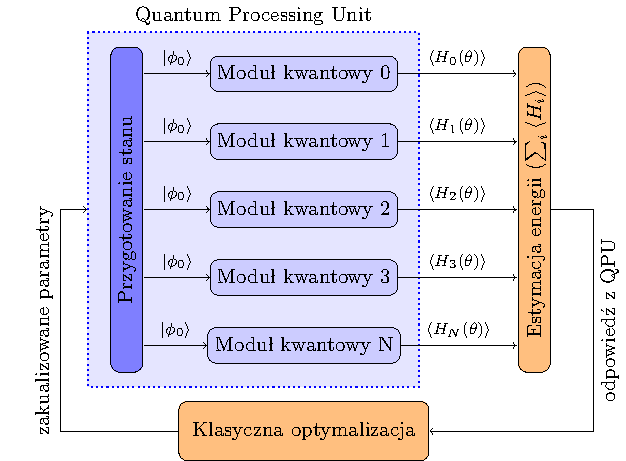
\includegraphics{vqe-pl.pdf}
\caption{Koncepcja działania kwantowego algorytmu wariacyjnego}
\end{figure}



\hypertarget{literatura}{%
\paragraph{Literatura}\label{literatura}}

\begin{enumerate}
\def\labelenumi{\arabic{enumi}.}
%\tightlist

\item Cerezo, M., Arrasmith, A., Babbush, R., Benjamin, S.C., Endo, S., Fujii, K., McClean, J.R., Mitarai, K., Yuan, X., Cincio, L. and Coles, P.J., 2021. Variational quantum algorithms. Nature Reviews Physics, 3(9), pp.625-644. \url{https://doi.org/10.1038/s42254-021-00348-9}

\item Tilly, J., Chen, H., Cao, S., Picozzi, D., Setia, K., Li, Y., Grant, E., Wossnig, L., Rungger, I., Booth, G.H. and Tennyson, J., 2022. The variational quantum eigensolver: a review of methods and best practices. Physics Reports, 986, pp.1-128. \url{https://doi.org/10.1016/j.physrep.2022.08.003}

\item \url{https://pennylane.ai/}

\item \url{https://qmlsys.mit.edu/}

\item 
\end{enumerate}

\end{document}
